\documentclass[article,colorback,accentcolor=tud4c]{tudreport}
\usepackage{ngerman}

\usepackage[stable]{footmisc} 
\usepackage[ngerman]{hyperref}
\usepackage[utf8]{inputenc}
\usepackage{longtable}
\usepackage{multirow}
\usepackage{booktabs}
\usepackage{pst-all}
\usepackage{amsmath}




% Makros
\newcommand{\before}[1]{\textit{ before(#1) }}
\newcommand{\after}[1]{\textit{after(#1)}}
\newcommand{\aktiv}[1]{\textit{active(#1)}}
\newcommand{\Interval}[1]{\textbf{interval#1}}
\newcommand{\comp}[1]{\textit{comp(#1)}}

\hypersetup{%
  pdftitle={TUD Corporate-Design f"ur {\LaTeX}}, pdfauthor={C. v. Loewenich und
  J. Werner}, pdfsubject={Beispieltext}, pdfview=FitH, pdfstartview=FitV }

\setcounter{seclinedepth}{1}

  \newif\ifTUDmargin\TUDmarginfalse \ifTUDmargin\makeatletter
    \TUD@setmarginpar{2}
  \makeatother\fi

\newlength{\longtablewidth}
\setlength{\longtablewidth}{0.7\linewidth}
\addtolength{\longtablewidth}{-\marginparsep}
\addtolength{\longtablewidth}{-\marginparwidth}

\title{IntervalEvents in EScala: Design}
\subtitle{Michael Kutschke und Frank Englert}


\begin{document}

\maketitle

\tableofcontents

\section{Todos}
\begin{enumerate}
  \item Dokumentation der Beispiele
  \item Dokumentation der Implmentierung
  \item Finden des Missing-Deploy-Bugs 
\end{enumerate}

\section{Grundlegende Definitionen}
Sei \before{\Interval} : Event das Ereignis, das den Beginn des Intervalls int angibt
und \after{\Interval} : Event jenes, welches das Ende von int angibt. Dies kann in
unterschiedlicher Form erfolgen:
\begin{itemize}
\item einmal \before{\_} zu Beginn und einmal \after{\_} am Ende (Standard in der jetzigen Fassung)
\item mehrfaches \before{\_} und ein \after{\_} am Ende (Use case? Wohl meist nicht erw"unscht)
\item verschachtelte, paarweise passende \before{\_} und \after{\_} Ereignisse (Bsp. Exec)
\item beliebige \before{\_} und \after{\_} Events innerhalb des Intervals
\end{itemize}
Ausserdem gebe \aktiv\Interval{} : boolean an, ob das Intervall aktiv ist.
In der jetzigen Fassung bedeutet dies einfach, ob man sich zeitlich innerhalb des
Intervalls befindet. Das Umschalten wude bisher als Sink realisiert. Dies führt
jedoch zu Indeterminismus, sodass e \&\& within(between(e,e')) beim ersten Vorkommen 
von e nicht unbedingt immer ausgeführt wird. Dies ist unschön und sollte vermieden werden.

Daher sollte active eine andere Semantik erhalten und als reaction aktualisiert
werden. So kann sichergestellt werden, dass der Zustand von active zu jedem
Zeitpunkt bekannt ist. Die Semantik ändert sich also wie in Abbildung
\ref{active_bit_behaviour} gezeigt. Dies ist keine Einschränkung, wie im
weiteren gezeigt werden wird.

\begin{figure}[h]
 \centering 
\psset{unit=1cm}
\begin{pspicture}(0,0)(10,2)
\psgrid[subgriddiv=1,griddots=10,gridlabels=7pt,](0,0)(10,2)
%{
%	\pspolygon[fillcolor=greenyellow,fillstyle=solid,linestyle=none](0,0)(0,1)(1,1)(1,0)

	\rput(1.2,1.7){\psframebox*[framearc=.3]{B}}
	\rput(9.2,1.7){\psframebox*[framearc=.3]{A}}
	\rput(0.2,1.55){\psframebox*[framearc=.3]{Früher}}
	\psline[linewidth=1pt]{[-]}(1,1.5)(9,1.5)

	\rput(1.2,0.7){\psframebox*[framearc=.3]{B}}
	\rput(9.2,0.7){\psframebox*[framearc=.3]{A}}
	\rput(0.2,0.55){\psframebox*[framearc=.3]{Aktuell}}
	\psline[linewidth=1pt]{]-]}(1,0.5)(9,0.5)
%}
\end{pspicture}
\caption{Wert des Aktiv-Bits}
\label{active_bit_behaviour}
\end{figure}


Für alle Intervalle muss gelten, dass active nur bei einem \before{\_} oder
\after{\_} Event umgeschaltet wird, wobei \aktiv{\_} nur von einem \before{\_}
Event gesetzt und von einem \after{\_} Event zurückgesetzt werden kann.
Ausserdem sollten ausserhalb des Intervalls keine isolierten Events auftreten.

\section{Operatoren}
Im folgenden werden einige Operatoren sowie ihre mögliche Imlementierung und
evtl. Schwächen des jeweiligen Ansatzes diskutiert.

\subsection{Komplement comp\Interval : Intervall}
\begin{itemize}
\item \before{\comp{\Interval}} <=> \after{\Interval}
\item \after{\comp{\Interval}} <=> \before{\Interval} \&\& ! \aktiv{\Interval}
\item \aktiv{\comp{\Interval}} <=> ! \aktiv{\Interval}
\end{itemize}
Probleme: An den Schnittpunkten ist ein Event laut dieser Definition sowohl in
int als auch \comp{\Interval}. Bei verschachtelten Events gibt es unerwünschte,
isolierte before(\comp{\Interval})-Events.

mögliche Lösungen: Komplement als Methode von Intervall Event überladbar
machen, und in Spezialfällen gesondert behandeln. Für das Schnittpunkt-Problem
gibt es (noch) keine Lösung, ist evtl. auch positiv (siehe Differenz)

Bemerkung: die zusätzlichen Bedingungen an after und active existieren aufgrund
der Nicht-Standard-Intervalle. Die explizite Definition von active ist wichtig damit das Komplement auch anfangs aktiv sein kann.

\subsection{Vereinigung \Interval{1} || \Interval{2} : Intervall}
Die Semantik der ||-Vereinigung soll eine Vereinigung der Zeitpunkte von \Interval{1}
und \Interval{2} sein, also w"are, falls \Interval{1} ein Exec Event wäre, \Interval{1} || \Interval{1} ein Standard Intervall.
\begin{itemize}
\item \before{\Interval{1} || \Interval{2}}  <=> (\before{\Interval{1}} ||
\before{\Interval{2}}) \&\& !
\aktiv{\Interval{1} || \Interval{2}}
\item \after{\Interval{1} || \Interval{2}} <=> ((\before{comp(\Interval{1})}
\&\& ! \aktiv{\Interval 2}) || (\before{\comp{\Interval{2}}} \&\& !
\aktiv{\Interval{1}}) || (\before{\comp{\Interval{1}}} \&\&
\before{\comp{\Interval{2}}})) \textbackslash \before{\Interval{1} ||
\Interval{} 2}
\end{itemize}
Anmerkung: statt \after{\Interval{1}} wurde hier \before{\comp{\Interval{1}}}
verwendet. In der jetzigen Fassung ist dies "aquivalent, allerdings bietet diese Formulierung den
Vorteil, dass falls die Probleme für Komplement gelöst werden, auch zum größten
Teil die Probleme mit Vereinigung verschwinden.

Problem: Verschachtelte Events, äahnlich wie bei Komplement. Eine Lösung für
das Problem mit Komplement löst auch dieses Problem.

\subsection{Schnitt \Interval{1} \&\& \Interval{2} : Intervall}
\begin{itemize}
\item \before{\Interval{1} \&\& \Interval{2}} <=> (((\before{\Interval{1}} \&\& \aktiv{\Interval{2}}) ||
(\before{\Interval{2}} \&\& \aktiv{\Interval{1}}) || (\before{\Interval{1}} \&\& \before{\Interval{2}}))
\textbackslash (\after{\Interval{1}} || \after{\Interval{2}})) \&\& ! \aktiv{\Interval{1} \&\& \Interval{2}}
\item \after{\Interval{1} \&\& \Interval{2}} <=> \before{\comp{\Interval{1}}} ||
\before{\comp{\Interval{2}}}
\item \aktiv{\Interval{1} \&\& \Interval{2}} <=> \aktiv{\Interval{1}} \&\& \aktiv{\Interval{2}}
\end{itemize}
Anmerkungen: zu \before{\comp{\_}} siehe Anm. zur Vereinigung

\subsection{Differenz \Interval{1} \textbackslash\ \Interval{2} : Interval}
Alle Zeitpunkte, die in \Interval{1} liegen, nicht aber in \Interval{2} (ausser Start bzw.
Endzeitpunkt, siehe Anm.). Wegen dieser Einschränkung kann es sinnvoll sein,
eine Bedingung an einen Zeitpunkt über eine Verbindung von within und !within
auszudrücken.

\Interval{1} \textbackslash\ \Interval{2} <=> \Interval{1} \&\& comp(\Interval{2})

Anmerkung: Wie bei Komplement erwähnt, sind die Eckpunkte von \Interval{1} und \Interval{2}
evtl. fälschlicherweise mit in \Interval{1} \textbackslash\ \Interval{2}. Dies
lässt sich nicht lösen, solange keine Möglichkeit gefunden wird, offene Intervalle zu
modellieren (z.B. über explizite before-Trigger o.ä.). U.U. ist dies aber auch
keine schlechte Eigenschaft, so dass ein Wechsel int -> \comp{\Interval{}}
atomar zu einem bestimmten Zeitpunkt stattfindet.

\subsection{within(\Interval{},e) : Event}
within(\Interval{},e) <=> (e \&\& \aktiv{\Interval}) || (e \&\& \before{\Interval})

\subsection{!within(\Interval{},e) : Event}
!within(\Interval{},e) <=> (e \&\& ! \aktiv{\Interval}) \textbackslash\ \before{\Interval}

\subsection{ StrictlyWithin(\Interval{},e) : Event}
StrictlyWithin(\Interval{},e) <=> (e \&\& \aktiv{\Interval}) \textbackslash\ \after{\Interval}

\subsection{ !strictlyWithin(\Interval{},e) : Event }
!strictlyWithin(\Interval{},e) <=> (e \&\& ! \aktiv{\Interval}) || (e \&\& \after{\Interval})

Problem: Auch hier werden bei verschachtelten Intervallen multiple \after{\_} Events mit aufgenommen.

\subsection{weitere Anmerkungen}
Der Umstand, dass sich int und \comp{\Interval{}} zwei Zeitpunkte teilen, mag
unintuitiv erscheinen, allerdings  bietet dies nicht nur Nachteile. So ist int
|| \comp{\Interval{}} wie  erwartet immer aktiv, beginnt und endet niemals. int
\&\& \comp{\Interval{}} ist niemals aktiv  und löst auch niemals before oder
after Ereignisse aus.

  \section{An Events gebundene Werte}
Es ist möglich, beliebige Werte an Events zu binden. Diese Möglichkeit soll
auch für Intervall-Events existieren. Wann im Intervall welche Werte gelten,
hängt von der Art des Intervalls ab. 

Auf den aktellen Wert des Intervalls wird über die Eigenschaft val zugegriffen.
Wenn also nachfolgend <Intervall>.val geschrieben steht, soll auf den aktuellen
Wert des Intervall-Events zugegriffen werden.

Nachfolgend wird das Standartverhalten der Intervall-Operatoren dargestellt.
Natürlich kann das Verhalten der Operatoren bei Bedarf abgeändert werden. Dann
muss beim Intervall-Event-Knoten eine Benutzerdefinierte Merge-Funktion
angegeben werden, die Values der Events aggregiert.

\subsection{Intervall zwischen dem Event B und dem Event A)}
Für between-Intervalle wie in Abbildung \ref{interval-between_b_a} gilt der Wert des
Before-Events bis zum End-Event. Dannach hat das Intervall den Wert null. Wenn der Wert des After-Events benötigt
wird, kann dieser über das Komplement des Intervalls erhalten werden. Beim
Intervall\ref{interval-between_b_a} gilt also:
\[
val(t) = \begin{cases}
null & t < 1 \\
B.val & t >= 1 \; and \; t < 9 \\
null & t >= 9
\end{cases}
\]

\begin{figure}[h]
 \centering 
\psset{unit=1cm}
\begin{pspicture}(0,0)(10,2)
\psgrid[subgriddiv=1,griddots=10,gridlabels=7pt](0,0)(10,1)
%{
%	\pspolygon[fillcolor=greenyellow,fillstyle=solid,linestyle=none](0,0)(0,1)(1,1)(1,0)

	\rput(1.2,0.7){\psframebox*[framearc=.3]{B}}
	\rput(9.2,0.7){\psframebox*[framearc=.3]{A}}
	\psline[linewidth=1pt]{[-]}(1,0.5)(9,0.5)
%}
\end{pspicture}
\caption{Intervall-Event between(B,A)}
\label{interval-between_b_a}
\end{figure}



Wenn die \before{\_}-Events mehrfach auftreten, hat das
between-Intervall als Wert den Wert des ersten \before{\_} oder des ersten
\after{\_}-Events. Ein Beispiel hierfür ist in Abbildung
\ref{interval-between_b_a-multiple} zu sehen. Für
Interval\ref{interval-between_b_a-multiple} gilt \[ val(t) =
\begin{cases}
null & t < 1\\
B.val &  t >= 1 \; and \; t < 7\\
null  & t >= 7
\end{cases}
\]

Für das
Komplement des Interval\ref{interval-between_b_a-multiple} gilt:
\[
comp.val = \begin{cases}
null & t < 7\\
A.val & t >= 7
\end{cases}
 \]
\begin{figure}[h]
 \centering 
\psset{unit=1cm}
\begin{pspicture}(0,0)(10,2)
\psgrid[subgriddiv=1,griddots=10,gridlabels=7pt](0,0)(10,1)
%{
	\rput(1.2,0.75){\psframebox*[framearc=.3]{B}}
	\rput(7.2,0.75){\psframebox*[framearc=.3]{A}}
	\psline[linewidth=1pt]{[-]}(1,0.5)(7,0.5)
	
	\rput(3.2,0.75){\psframebox*[framearc=.3]{B'}}
	\rput(9.2,0.75){\psframebox*[framearc=.3]{A'}}
	\psline[linewidth=1pt,linestyle=dotted]{[-]}(3,0.5)(9,0.5)
%}
\end{pspicture}
\caption{Intervall-Event between(B,A) mit mehrfach auftretenden Before- und
After-Events}
\label{interval-between_b_a-multiple}
\end{figure}
 
 
\subsection{Vereinigung von Intervallen}
Für die Vereinigung von Intervallen ist es sinnvoll, den Wert des letzen
\before{\_}-Events zu speichern. Damit hat man immer Zugriff auf den Wert des
letzten Events, der die Bedingung erfüllt hat. 

\begin{figure}[h]
 \centering 
\psset{unit=1cm}
\begin{pspicture}(0,0)(10,4)
\psgrid[subgriddiv=1,griddots=10,gridlabels=7pt](0,0)(10,3)
%{
	\rput(1.2,2.75){\psframebox*[framearc=.3]{B}}
	\rput(7.2,2.75){\psframebox*[framearc=.3]{A}}
	\psline[linewidth=1pt]{[-]}(1,2.5)(7,2.5)
	
	\rput(3.2,1.75){\psframebox*[framearc=.3]{B'}}
	\rput(9.2,1.75){\psframebox*[framearc=.3]{A'}}
	\psline[linewidth=1pt]{[-]}(3,1.5)(9,1.5)
	
	\rput(1.2,0.75){\psframebox*[framearc=.3]{B}}
	\rput(9.2,0.75){\psframebox*[framearc=.3]{A'}}
	\psline[linewidth=1pt]{[-]}(1,0.5)(9,0.5)
%}
\end{pspicture}
\caption{Vereinigung zweier Intervall-Events: between(B,A) || between(B',A')}
\label{interval-or}
\end{figure}
  
Für das in Abb\ref{interval-or} zu sehende Interval\ref{interval-or}
between(A,B) || between(A',B') gilt also die folgende Belegung des Wertes:
\[
val(t) = \begin{cases}
null & t < 1 \\
A.val & t >=1 \; and t < 3 \\
A'.val & t >=3 \; and t < 9 \\
null & t > 9 \\
\end{cases}
\]

Und für das Komplement von Interval\ref{interval-or} gilt die Belegung:
\[
val(t) = \begin{cases}
null & t < 9 \\
A'.val & t >= 9
\end{cases}
\]
  
  \subsection{Schnittmenge zwischen Intervallen}
Bei der Schnittmenge zwischen zwei Intervall-Events werden die Event-Werte der
beiden aktiven Interval-Events zu einem Tupel zusammengefasst. 

\begin{figure}[h]
 \centering 
\psset{unit=1cm}
\begin{pspicture}(0,0)(10,4)
\psgrid[subgriddiv=1,griddots=10,gridlabels=7pt](0,0)(10,3)
%{
	\rput(1.2,2.75){\psframebox*[framearc=.3]{B}}
	\rput(7.2,2.75){\psframebox*[framearc=.3]{A}}
	\psline[linewidth=1pt]{[-]}(1,2.5)(7,2.5)
	
	\rput(3.2,1.75){\psframebox*[framearc=.3]{B'}}
	\rput(9.2,1.75){\psframebox*[framearc=.3]{A'}}
	\psline[linewidth=1pt]{[-]}(3,1.5)(9,1.5)
	
	\rput(3.2,0.75){\psframebox*[framearc=.3]{(B,B')}}
	\rput(7.2,0.75){\psframebox*[framearc=.3]{(A', A)}}
	\psline[linewidth=1pt]{[-]}(3,0.5)(7,0.5)
%}
\end{pspicture}
\caption{Schnittmenge zweier Intervall-Events: between(B,A) and
between(B',A')}
\label{interval-and}
\end{figure}

Wie in Abb. \ref{interval-and} zu sehen, ergibt sich das folgende Zeitliche
Verhalten für den Wert von Interval\ref{interval-and} \[
val(t)=\begin{cases}
null & t < 3 \\
(B,B') & t >=3 \; and t <= 7 \\
null & t > 7
\end{cases}
\]

Das Komplement von Intervall \ref{interval-and} hat die Belegung: \[
val(t) = \begin{cases}
null & t <= 7\\
(A', A) & t > 7
\end{cases} 
\]

\subsection{Differenz zweier Intervall-Events}
Bei der Differenz zwischen zwei Intervall-Events ist der Wert des Intervalls das
letzte Before-Event vor oder nach dem Schnitt. Für de

\begin{figure}[h]
 \centering 
\psset{unit=1cm}
\begin{pspicture}(0,0)(10,4)
\psgrid[subgriddiv=1,griddots=10,gridlabels=7pt](0,0)(10,3)
%{
	\rput(1.2,2.75){\psframebox*[framearc=.3]{B}}
	\rput(4.2,2.75){\psframebox*[framearc=.3]{A}}
	\psline[linewidth=1pt]{[-]}(1,2.5)(4,2.5)
	
	\rput(6.2,2.75){\psframebox*[framearc=.3]{B''}}
	\rput(9.2,2.75){\psframebox*[framearc=.3]{A''}}
	\psline[linewidth=1pt]{[-]}(6,2.5)(9,2.5)
	
	\rput(3.2,1.75){\psframebox*[framearc=.3]{B'}}
	\rput(5.2,1.75){\psframebox*[framearc=.3]{A'}}
	\psline[linewidth=1pt]{[-]}(3,1.5)(5,1.5)
	
	\rput(1.2,0.75){\psframebox*[framearc=.3]{B}}
	\rput(3.2,0.75){\psframebox*[framearc=.3]{B'}}
	\psline[linewidth=1pt]{[-]}(1,0.5)(3,0.5)
	
	\rput(6.2,0.75){\psframebox*[framearc=.3]{B''}}
	\rput(9.2,0.75){\psframebox*[framearc=.3]{A''}}
	\psline[linewidth=1pt]{[-]}(6,0.5)(9,0.5)
%}
\end{pspicture}
\caption{Schnittmenge zweier Intervall-Events: between(B,A) and
between(B',A')}
\label{interval-diff}
\end{figure}

Für Interval\ref{interval-diff} ergibt sich also folgende Belegung:
\[
val(t)=\begin{cases}
null & t < 1 \\
B & t \in [1,3] \\
null & t \in [3,6] \\
B'' & t\in[6,9]\\
null & t >9
\end{cases}
\]

Für das Komplement von Interval\ref{interval-diff} ergibt sich der zeitliche
Werteverlauf:\[
val(t)= \begin{cases}
null & t < 3\\
B' & t \in [3,5]\\
null & t > 6
\end{cases}
\]

\section{Beispiele}

Das Ziel dieses Abschnittes ist es, dem Benutzer die Verwendung von
Intervall-Events näherzubringen. Dazu wird gezeigt, an welchen Stellen sich
Intervall-Events sinnvoll einsetzen lassen. Bis auf das letzte Beispiel
existieren für alle Beispiele zwei Implementierungen. Eine Implementierung die
Intervall-Events verwendet und eine Implementierung die keine Events
verwendet.

\subsection{Implementierung eines Zustandsautomaten}
Zwei Beispiele zeigen die Verwendung von Intervall-Events bei der
Implementierung von Zustandsautomaten. Zustandsautomaten k"onnen hervoragend
durch die Verwendung von IntervallEvents implementiert werden, da
Zustandsautomaten immer vom Zustand abh"anige Reaktionen auf Events zeigen.

Zur Implementierung kann jeder Zustand des Automaten als ein Intervall
abgebildet werden. Alle in einen Zustand eingehende Transitionen werden dabei
als Start-Events des Intervalls verwendet und alle vom Zustand ausgehende
Transitionen werden als End-Event des Intervalls verwendet. Alternativ könnte
man auch die \after{}-Events des vorherigen Zustandsintervalls als Startevent
des nächsten Zustandes verwenden.

Durch diese Vorgehensweise ergibt sich eine bessere Wartbarkeit des
Quellcodes, da das Programmverhalten nicht mehr imperativ durch If-Statements
oder das Statemachine-Pattern beschrieben wird. Viel mehr wird das
Programmverhalten deklarativ durch Intevall-Events spezifiziert.

Im Rahme dieser Arbeit wurden zwei Zustandsautomaten implementiert. Der erste
Zustandsautomat besteht aus zwei Zuständen und soll dem Benutzer die
Vorgehensweise zur Implementierung eines Zustandsautomaten an einem stark
vereinfachten Beispiel zeigen. Der resultierende Zustandsautomat ist in Abb.
\ref{filetransfer_behaviour} zu sehen.

%\usepackage{graphics} is needed for \includegraphics
\begin{figure}[htp]
\begin{center}
  \includegraphics[width=0.15\textwidth]{graphics/tcp_stm.dot.eps}
  \caption{Verhalten einer Filetransfer-Verbindung}
  \label{filetransfer_behaviour}
\end{center}
\end{figure}


Im SimpleWebshop-Beispiel wird eine weitere Herangehensweise an die
Implementierung eines Zustandsautomaten mit Intervall-Events gezeigt. Häufig
lässt sich die Anzahl der benötigten Zustände und Transitionen durch die
Verwendung von paralellen oder hierarchischen Zustandsautomaten reduzieren.
Damit wird das Modell leichter verständlich aber die Implementierung des Modells
erschwert. 
Besonders die Implementierung von paralellen Zustandsautomaten ist zumeist sehr
unpraktisch. Der Zugriff auf den aktuellen Zustand der paralellen
Zustandsautomaten und das Verteilen von Events bereitet nämlich meist
Probleme. Daher werden oft zur Implementierung die Produktautomaten gebildet um
die paralellen Zustände aus dem Modell zu entfernen.

Dies ist bei der Verwendung von Intervall-Events zur Impelmentierung eines
Zustandsautomaten allerdings nicht zwingend notwendig. Die direkte
Implementierung eines paralellen Zustandsautomaten ist ohne Probleme möglich.
Die Verteilung der Events zum Ändern der Zustände und der Zugriff auf
benachbarte Zustandsautomaten ist einfach. 

Die Implementierung eines solchen Zustandsautomaten wie in Abb.
\ref{webshop_behaviour} dargestellt findet sich im Beispiel
interval\_simplewebhop.

%\usepackage{graphics} is needed for \includegraphics
\begin{figure}[htp]
\begin{center}
  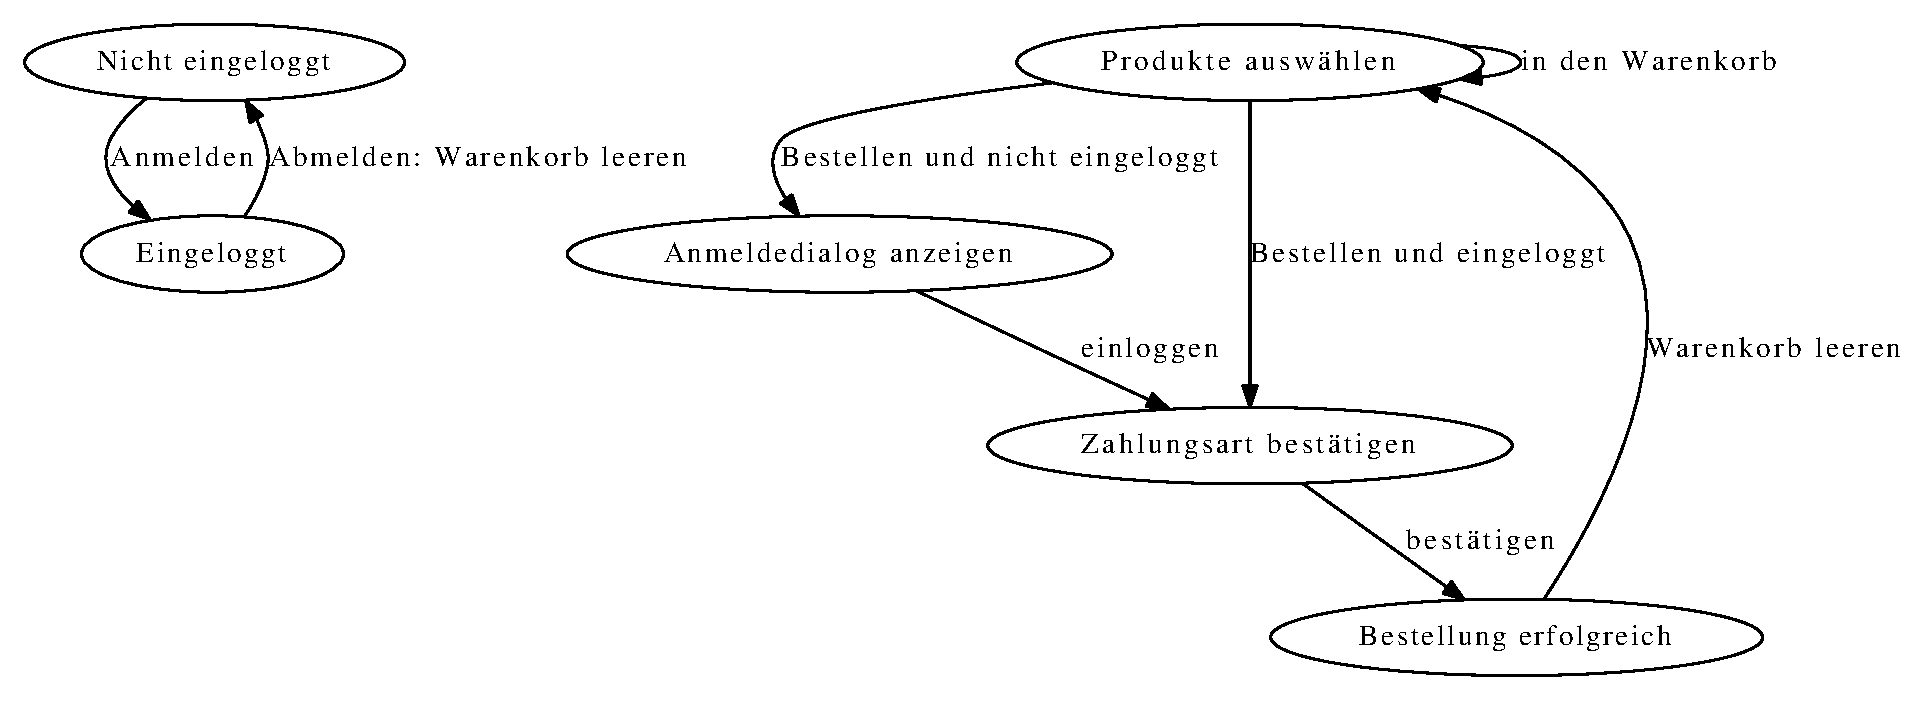
\includegraphics[width=0.6\textwidth]{graphics/webshop.dot.eps}
  \caption{Bestellvorgang in einem Web-Shop}
  \label{webshop_behaviour}
\end{center}
\end{figure}

\subsection{Implementierung einer FileTransfer-Komponente}
In viele Fällen wird ein Softwareentwickler keinen Zustandsautomaten
spezifizieren bevor die Software-Entwicklung beginnt. Viele zu lösende Probleme
lassen sich nämlich durch zwei oder drei Zustände beschreiben, sodass der
Entwickler nicht erst auf die Idee kommt, eine Zustandsmaschine zu
implementieren. Daher stellt sich die Frage, ob Intervall-Events auch in der
Praxis relevant sich um dem Entwickler beim Lösen von alltäglichen Problemen zu
helfen. Das nächste Beispiel zeigt daher die praktische Verwendung von
Intervall-Events:

Mit File-Sharing-Programmen können Benutzer über ein Computernetzwerk
Dateien austauschen. Wenn ein Benutzer eine Dateiübertragung anfordert, dann
fordert das File-Sharing-Programm von unterschiedlichen Hosts Teile der Datei
an. Die Hosts anworten dann mit den angeforderten Dateiteilen. Daher existiert
in den meisten File-Sharing-Programmen eine Komponente zum Steuern der
Dateiübertragungen. Diese Komponente verwaltet die bereits empfangenen
Dateiteile und kümmert sich darum, noch fehlende Tokens nachzufordern.

Bei der Implementierung einer solchen Komponente bietet sich die Verwendung von
Intervall-Events an. Das Verhalten der FileTransfer-Komponente kann fast
vollständig deklarativ erfolgen. 

\subsection{Implementierung von Ping-Pong}
Als größeres Beispiel wurde im Rahmen des Praktikums das Spiel
Ping-Pong implementiert. In diesem Spiel gibt es ein abgegrenztes Spielfeld mit
Wänden. Im Spielfeld befindet sich ein Ball der sich bewegt. Am Spiel teil
nehmen zwei Spieler die jeweils einen eindimensional beweglichen Schläger haben.
Der Schläger befindet sich vor dem Tor des Spielers. Ziel des Spiels ist es, den
Ball nicht in das eigene Tor zu lassen. Als kleine Erweiterung erscheinen auf
der Spielfläche Geschenke die das Spielverhalten abändern. Die Spielfläche des
Spiels ist in Abb. \ref{ping_pong} zu sehen.

\begin{figure}[htp]
\begin{center}
  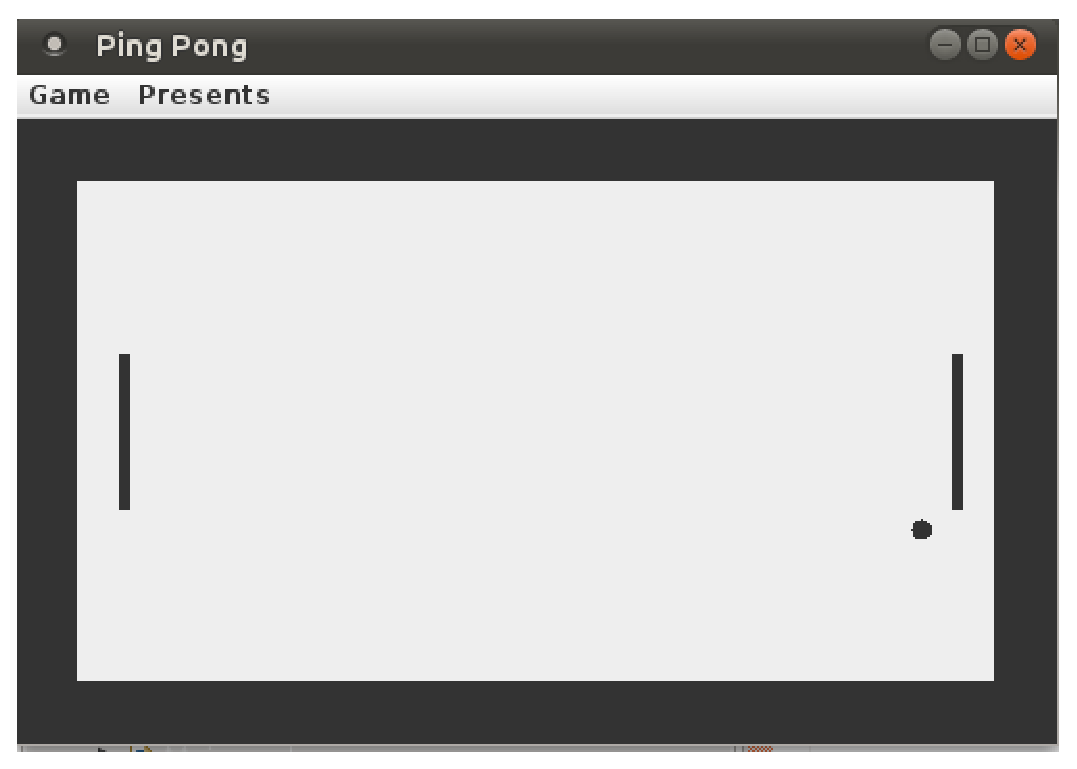
\includegraphics[width=0.6\textwidth]{graphics/pingpong.eps}
  \caption{Ping-Pong}
  \label{ping_pong}
\end{center}
\end{figure}

Das Spielmodell beinhaltet die Wände, den Ball, die Schläger, die Tore und
eventuell Geschenke. Jedes Objekt auf dem Spielfeld hat eine Position und eine
Geschwindigkeit. Allerdings wurde bei der Implementierung des Spiels von der
Klassischen Herangehensweise abgewichen. Klassischerweise besteht ein Spiel aus
einer Spielschleife in der die folgenden Aktionen immer wieder ausgeführt
werden:
\begin{itemize}
  \item Abfragen der Benutzereingaben
  \item Berechnung der Änderungen im Spiel-Modell. Also die Positionsänderung
  des Balls und der Schläger.
  \item Rendern des Spielmodells zu einer Grafik
  \item Warten bis die nächste Iteration notwendig wird. Ohne diese Wartezeit
  hätte man möglicherweise eine zu hohe Frame-Rate.
\end{itemize}

Diese Ansatz ist allerdings nicht Event-Orientiert und wurde daher im Beispiel
nicht verwendet. Stattdesen wird im Beispiel ein Timer verwendet, der alle 50ms
eine Positionsänderung der Objekte und und das Neuzeichnen der Spielfläche auslöst.
Solange ein Spieler eine Bewegen-Taste drückt ist ein Intervall-Event aktiv das
die Geschwindigkeit des Schlägers ändert\footnote{Dies ist übrigens ein
eleganter Workaround für einen Bug in der Java AWT. Mehr Informationen zum
diesem Fehler finden sich unter
bugs.sun.com/view\_bug.do?bug \_id=4153069}.

Weiterhin werden Intervall-Events eingesetzt, um das Zeitmodell des Spiels
abzubilden. Geschenke beispielsweise sollen nur für eine definierte Zeit
vorhanden sein. Diese Funktion wurde durch ein Intervall-Event realisiert, das
vom Beginn der Sichtbarkeit für eine gewisse Zeit aktiv ist. 

\subsection{Zusammenfassung}
Fasst man die Beispiele zu einem Fazit zusammen, so lässt sich sagen, dass durch
die Verwendung von Intervall-Events ein deklaratives Implementieren von
zustandsbasierten Problemen möglich ist. Dies verbessert die Lesbarkeit und die
Wartbarkeit des Quellcodes. Allerdings gibt müssen zwei Schwierigkeiten bei der
Verwendung von Intervall-Events bedacht werden: Zum einen ist Vorsicht bei der
Verwendung von rekursiven Definitionen geboten. Eine Verwendung dieser
Konstrukte erfordert das Markieren des Start-Intervalls mit \textit{lazy} und
die Definition eines Startevents um eine korrekte Initialisierung der rekursiven
Definition vorzunehmen.

Zum anderen ist es wichtig, ein exaktes Event-Modell für eingehende und
ausgehende Events zu erstellen. Es ist wichtig, zwischen Events die Transitionen
auslösen können und Events die Aktionen zur Folge haben zu trennen. Ist diese
Trennung nicht exakt genug, dann könnten eventuell Aktionen ausgeführt werden,
die im akutellen Intervall nicht zulässig sind. 

Beachtet man diese Entwurfskriteren, so ist es durch Intervall-Events möglich,
auf einem hohe Abstraktionsnivea Software zu entwicklen. 



\listoffigures\addcontentsline{toc}{section}{\listfigurename}
\end{document}
